% ===============================================================
\section{Part 1 -- Nucleate boiling of a water/2-propanol mixture in variable gravity}
% ===============================================================

\subsection{Task 2.1 -- Data preparation and first look at the data}
\label{sec:t21}

\paragraph{(a) Installation and check of the data array.}
\code{CodeP2.1F26} was run in the first cell of the notebook \code{P2\_Task2.1.ipynb}. It prints
the array \code{ydata} (45 rows $[\qpp,\ T_w-T_{sat},\ g,\ \gamma,\ P]$, those printed in black in
the Appendix) and a single element. Instead of comparing the printed array with the Appendix by eye,
I wrote a small check program (cell~3). It reads all the rows of the original skeleton file (active
and commented-out lines, 77 rows) and compares them, row by row, with the Appendix listing typed from
the project statement. \textbf{Two rows of the skeleton code do not match the Appendix}
(Table~\ref{tab:datacheck}). Both rows are in the active $g=0.098$~m/s$^2$ group. I corrected them to the
Appendix values in all my programs. After the correction, the 45 active rows agree exactly with the
Appendix, and the single element \code{ydata[3][0]} $=59.2$ is the 4th heat flux of the listing, as
expected (indices start at 0).

\begin{table}[H]
\centering\small
\caption{Differences between the data of the skeleton program \code{CodeP2.1F26} and the Appendix of the statement.}
\label{tab:datacheck}
\begin{adjustbox}{max width=\linewidth}
\begin{tabular}{@{}c l l l@{}}
\toprule
Row (index) & Skeleton code & Appendix & Correction applied\\
\midrule
0 & \code{[44.2, 32.5, 0.098, 1.79, 5.5]} & \code{[44.1, 32.5, 0.098, 1.79, 5.5]} & $\qpp$: $44.2\to44.1$ W/cm$^2$\\
6 & \code{[76.3, 37.8, 0.098, 1.79, 5.5]} & \code{[76.3, 37.5, 0.098, 1.79, 5.5]} & $T_w-T_{sat}$: $37.8\to37.5$\,\textdegree C\\
\bottomrule
\end{tabular}
\end{adjustbox}
\end{table}

\paragraph{(b) Log-log plot of heat flux versus superheat.}
Figure~\ref{fig:t21} shows the first two groups of the Appendix ($g=0.098$ and $9.8$~m/s$^2$,
$P=5.5$~kPa, $\gamma=1.79$). To quantify the trends, I fitted a power law $\qpp=C\dTsat^m$ to each group
(least squares on the logarithms):
\[
g=0.098~\text{m/s}^2:\ \qpp=\TwoOneClow\,\dTsat^{\TwoOneMlow},\quad
g=9.8~\text{m/s}^2:\ \qpp=\TwoOneChigh\,\dTsat^{\TwoOneMhigh}.
\]
Two observations guide the rest of Part~1:
\begin{itemize}
  \item The heat flux varies \textbf{strongly with superheat}. The exponent is close to 3, the classical
        value for nucleate boiling of pure fluids, so $n_2\approx3$ is a physically motivated initial guess.
  \item The heat flux varies \textbf{very weakly with gravity}. The two curves almost coincide:
        $\qpp(9.8)/\qpp(0.098)=1.05$, $1.01$ and $0.98$ at 32, 40 and 50\,\textdegree C, while $g$ changes by a
        factor of 100. For a pure fluid, $\qpp\sim g^{n}$ with $n\approx0.01$--$0.25$ would predict a
        decrease by a factor of about 1.5--3 between $1\,\gen$ and $0.01\,\gen$. This is the signature
        of the Marangoni effect described in the statement: at low gravity, the surface-tension-driven flow
        still brings liquid to the heated surface, so the heat flux does not drop. A simple power law in
        $g$ (Eq.~(1.1)) is therefore not expected to describe the gravity effect well.
\end{itemize}

\begin{figure}[H]
\centering
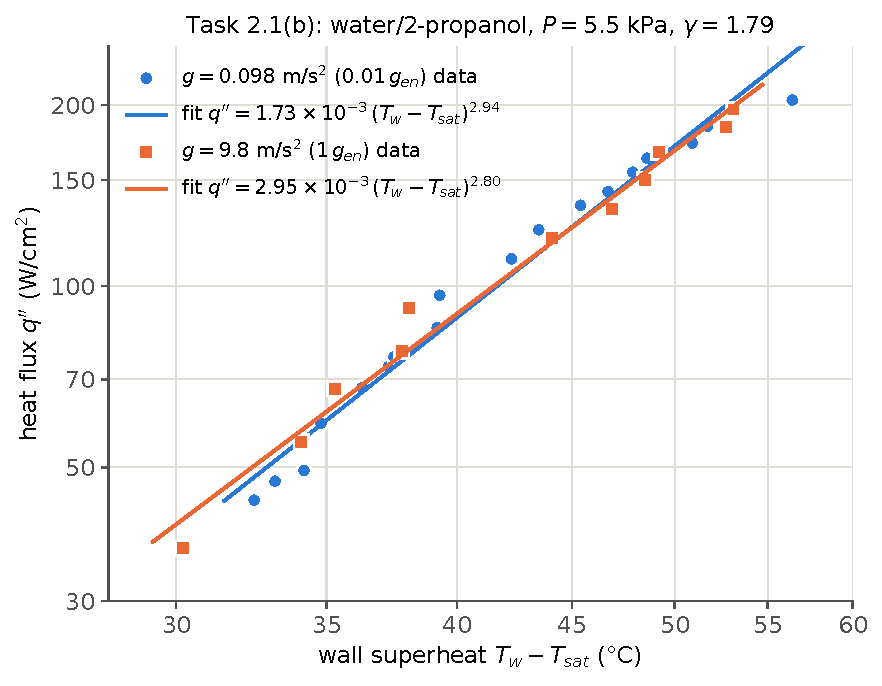
\includegraphics[width=0.66\linewidth]{figures/t21_loglog.pdf}
\caption{Task 2.1(b): heat flux versus wall superheat for $g=0.098$ and $9.8$~m/s$^2$ (log-log axes),
with a power-law fit for each gravity level.}
\label{fig:t21}
\end{figure}

% ---------------------------------------------------------------
\subsection{Task 2.2 -- Three-constant model $\qpp=n_1\dTsat^{n_2}g^{n_3}$}
\label{sec:t22}

\paragraph{Assembly of the program.}
\code{CodeP2.1F26} (data, corrected as above) and \code{CodeP2.2F26} were placed in two consecutive cells
of \code{P2\_Task2.2.ipynb}. \textbf{The program provided does not run as it is}: the line
\code{import random} at the top of \code{CodeP2.2F26} gives the name \code{random} to the
\emph{module} and hides the \emph{function} \code{random()} imported by \code{CodeP2.1F26}. The
initialisation \code{n1i+0.001*random()} then stops with
\code{TypeError: 'module' object is not callable}. I replaced it with \code{from random import random, seed}.
The other changes (Section~\ref{sec:codechanges}) do not modify the algorithm. The evolution loop is
placed in a function \code{run\_GA(n1i, n2i, n3i, NGEN, MUT, MFRAC, rseed)}, so that it can be re-run
for many initial guesses. The mutation amplitude (0.085 in the code) becomes the argument \code{MUT},
and both random generators are seeded.

\paragraph{First run (skeleton initial guesses).}
With the initial guesses of the skeleton ($n_1=0.00027$, $n_2=4.0$, $n_3=0.063$), MUT $=0.085$ and
NGEN $=6000$, $\Ferrmean$ drops below the target 0.035 after only \TwoTwoBaseKconv\ generations. The
minimum, $\Ferrmean=\TwoTwoBaseF$, is reached at generation \TwoTwoBaseKmin\ (first lines of
Table~\ref{tab:t22const}). The target is met. However, $n_2=3.34$ is far from the value
$n_2\approx3$ of Task~2.1(b), and a second look shows that this solution is not the best one.

\paragraph{Effect of the initial guesses, of the mutation amplitude and of NGEN.}
Four sets of initial guesses were tested (Table~\ref{tab:t22study}). Set~1 is the skeleton guess and
Set~2 a physics-based guess ($n_2=3$, $0.01<n_3<0.1$). Set~3 is far from the solution ($n_2=2$,
$n_3=0.25$) and Set~4 very far ($n_1$ about 1500 times too small, $n_2=5$). Each set was run with 5
different random seeds, for three maximum mutation amplitudes (MUT $=\pm8.5$, $\pm20$ and $\pm40\,\%$),
with a longer run (NGEN $=20000$), and with a two-stage strategy: exploration with MUT $=0.40$, then a
restart from the best constants with MUT $=0.03$. In total 88 runs were made.
Figure~\ref{fig:t22conv} shows the convergence histories and Figure~\ref{fig:t22land} the trajectories of
the population-average constants on the error landscape.

\begin{table}[H]
\centering\scriptsize
\caption{Task 2.2: effect of the initial guesses, of the maximum mutation amplitude MUT and of NGEN
(5 seeds per line, 2 for NGEN $=20000$). ``best/median/worst'' = minimum $\Ferrmean$ reached in a run;
``$<0.035$'' = number of runs that reach the target; $k_{0.035}$ = median generation at which the target is first
reached; last column = spread of the best-fit $n_2$ between seeds. Deterministic reference minimum:
$\Ferrmean=\TwoTwoRefF$ at $n_2=\TwoTwoRefNtwo$.}
\label{tab:t22study}
\fittable{t22_study}
\end{table}

\begin{figure}[H]
\centering
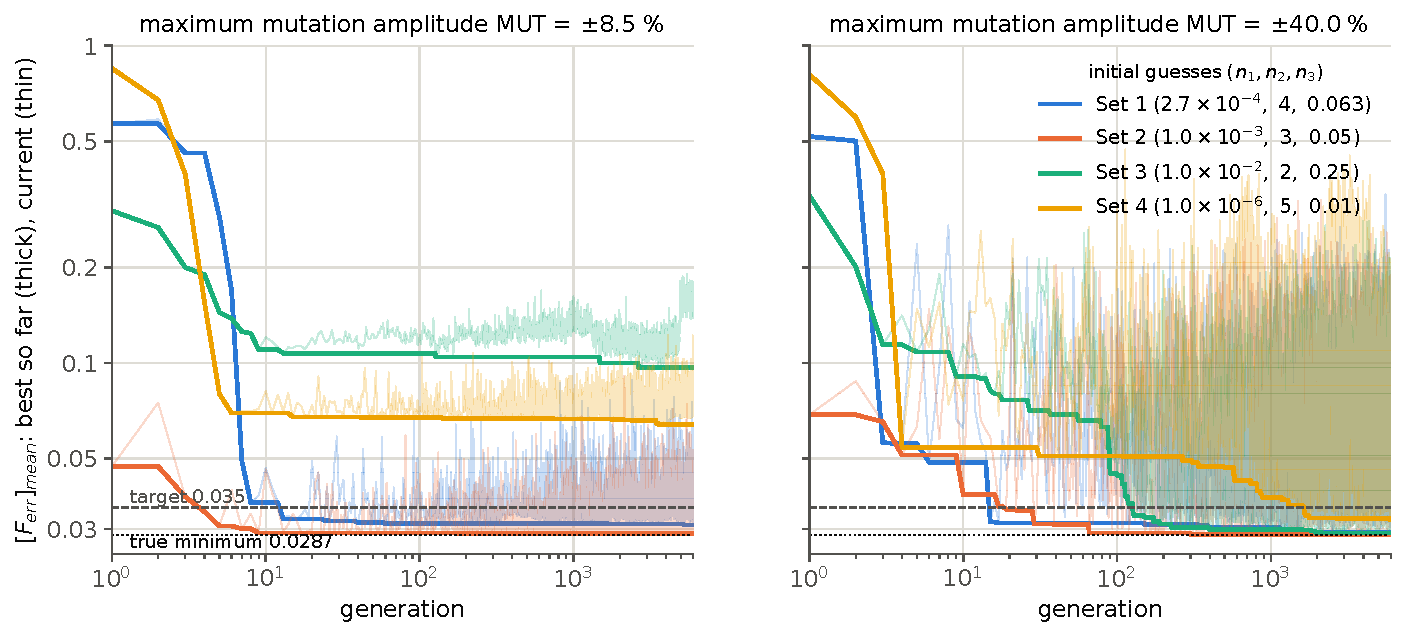
\includegraphics[width=\linewidth]{figures/t22_convergence.pdf}
\caption{Task 2.2: convergence of $\Ferrmean$ for the four sets of initial guesses (seed 1). Thick lines:
best value so far; thin lines: value at each generation. Left: skeleton mutation amplitude ($\pm8.5\,\%$);
right: $\pm40\,\%$.}
\label{fig:t22conv}
\end{figure}

\begin{figure}[H]
\centering
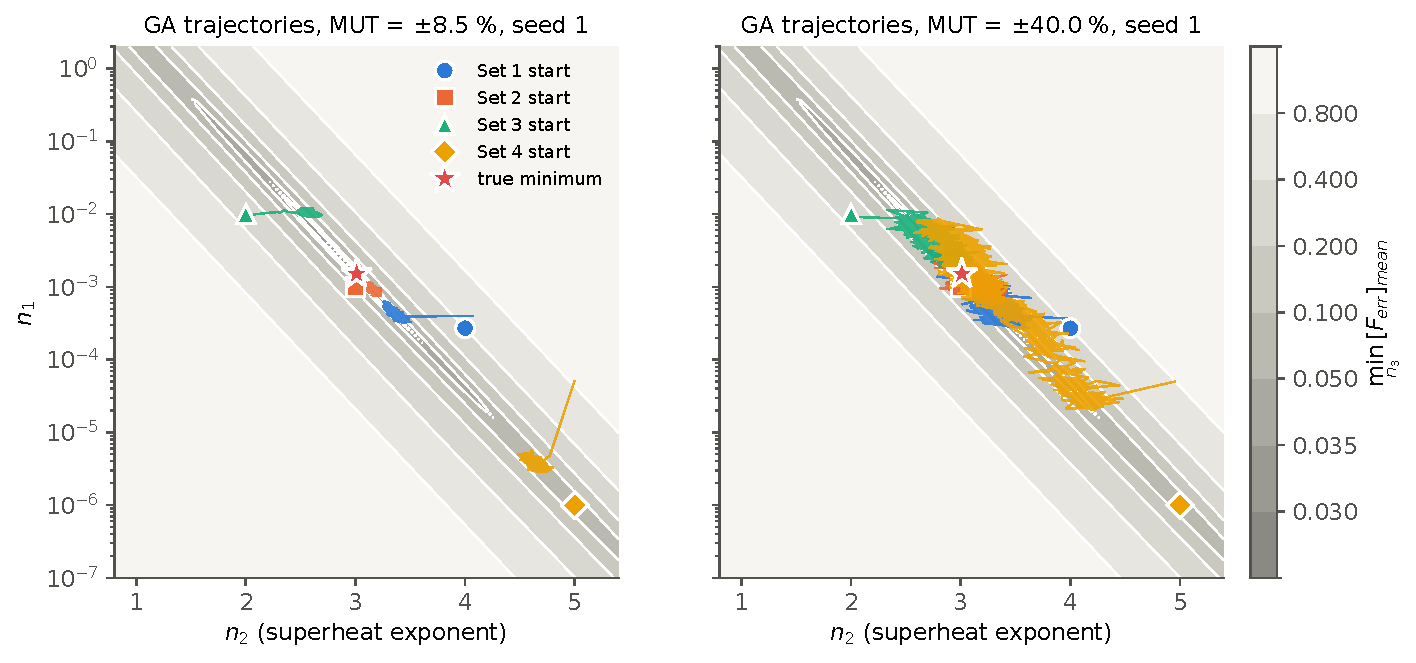
\includegraphics[width=\linewidth]{figures/t22_landscape.pdf}
\caption{Task 2.2: error landscape (minimum over $n_3$ of $\Ferrmean$ in the $(n_2,n_1)$ plane) and
trajectories of the population-average constants of the four sets (seed 1). The error has a long, narrow
valley along $\ln n_1+3.7\,n_2\approx\text{const}$.}
\label{fig:t22land}
\end{figure}

The main observations are:
\begin{itemize}
  \item \textbf{Guesses close to the solution (Sets 1 and 2) converge for every mutation amplitude and every
        seed}, in a few generations. The target 0.035 is reached after 2--12 generations, because the GA
        only has to adjust $n_1$ to the level of the data. Even so, with the skeleton amplitude
        ($\pm8.5\,\%$), Set~1 stops at $n_2=3.08$--$3.34$ depending on the seed. The error is below the target,
        but these constants are not the optimum.
  \item \textbf{The error surface is a narrow valley} (Fig.~\ref{fig:t22land}). Since
        $\ln\qpp=\ln n_1+n_2\ln\dTsat+n_3\ln g$ and $\ln\dTsat\approx3.7$ in the middle of the data,
        $\ln n_1$ and $n_2$ compensate each other: along the valley floor, $\Ferrmean$ stays below 0.035
        for $2.2\lesssim n_2\lesssim3.6$. A mutation of $\pm8.5\,\%$ on $n_2$ ($\pm0.26$) changes $\ln\qpp$
        by about $\pm1$, which is much more than the scatter of the data (about 0.15). As a result, almost only
        the offspring whose mutations of $n_1$ and $n_2$ compensate each other survive, and the population
        moves along the valley very slowly, like a random walk.
  \item \textbf{Far guesses (Sets 3 and 4) do not converge with the skeleton amplitude}, and giving
        them more generations does not help. With MUT $=0.085$, Set~3 reaches the target in only 1 run
        out of 5 and Set~4 never does. NGEN $=20000$ gives no improvement (0/2): the population remains trapped at $n_2\approx2.5$ with $n_3\approx0.2$
        (Set~3), or at $n_2\approx4.4$ (Set~4), with $\Ferrmean\approx0.06$--$0.10$. As suggested in the statement, \textbf{increasing the mutation
        amplitude solves the problem}. With $\pm40\,\%$, all runs of Sets~3 and 4 reach the target, after
        about 130 and 1600 generations. The cost is a much noisier population (thin lines in
        Fig.~\ref{fig:t22conv}), so the minimum is reached only occasionally.
  \item \textbf{The two-stage strategy (large mutations to explore, then small mutations to refine)
        combines robustness and accuracy.} It keeps the $100\,\%$ success rate of the $\pm40\,\%$ runs,
        even from Set~4. It lowers the median error of every set compared with the single $\pm40\,\%$ run,
        and it produced the overall best fit. For guesses that are already close to the solution, a
        moderate amplitude ($\pm20\,\%$) in a single run works just as well.
\end{itemize}

\paragraph{Best fit.}
The best of the 88 runs (\TwoTwoBestSet, two-stage, seed \TwoTwoBestSeed) gives the constants of
Table~\ref{tab:t22const}:
\[
\boxed{\qpp=\TwoTwoNone\,\dTsat^{\,\TwoTwoNtwo}\,g^{\,\TwoTwoNthree}}\qquad
\Ferrmean=\TwoTwoF\ (<0.035).
\]
This error is within $0.05\,\%$ of the true minimum of the error function ($\TwoTwoRefF$) found by the
deterministic check. The constants themselves differ slightly from the reference ($n_2$: $-1.2\,\%$,
$n_3$: $-6\,\%$, $n_1$: $+14\,\%$). This difference is the flat valley again: these sets of constants
describe the data equally well. The robust result is $n_2\approx3.0\pm0.05$ and a weak exponent
$n_3\approx0.045$.

\begin{table}[H]
\centering\small
\caption{Task 2.2: constants of Eq.~(1.1) printed by the program (MINIMUM = population-average constants
at the minimum of $\Ferrmean$, ENDING = last generation, TIME AVG = average over generations 801--NGEN).
$^\dagger$the TIME AVG error printed by the skeleton is the average of $\Ferrmean$ over all generations.}
\label{tab:t22const}
\fittable{t22_constants}
\end{table}

\paragraph{Predicted versus measured heat flux and rms deviation.}
Figure~\ref{fig:t22parity}(a) shows each pair $(\qpp_{pred},\qpp_{exp})$ as a discrete point on log-log
axes, with the line of slope 1 and the $\pm10\,\%$ lines. Figure~\ref{fig:t22parity}(b) shows the
fractional deviation for each gravity level. The deviation statistics are:
\begin{itemize}
  \item rms deviation of $\qpp_{exp}$ from $\qpp_{pred}$: $\TwoTwoRmsAbs$~W/cm$^2$ (mean heat flux
        $\TwoTwoMeanQ$~W/cm$^2$);
  \item rms fractional deviation $\sqrt{\overline{[(\qpp_{exp}-\qpp_{pred})/\qpp_{pred}]^2}}=\TwoTwoRmsRel\,\%$,
        mean absolute fractional deviation $\TwoTwoMeanAbsRel\,\%$, maximum $\TwoTwoMaxRel\,\%$;
  \item only $\TwoTwoWithin\,\%$ of the points are within $\pm10\,\%$ of the prediction.
\end{itemize}

\begin{figure}[H]
\centering
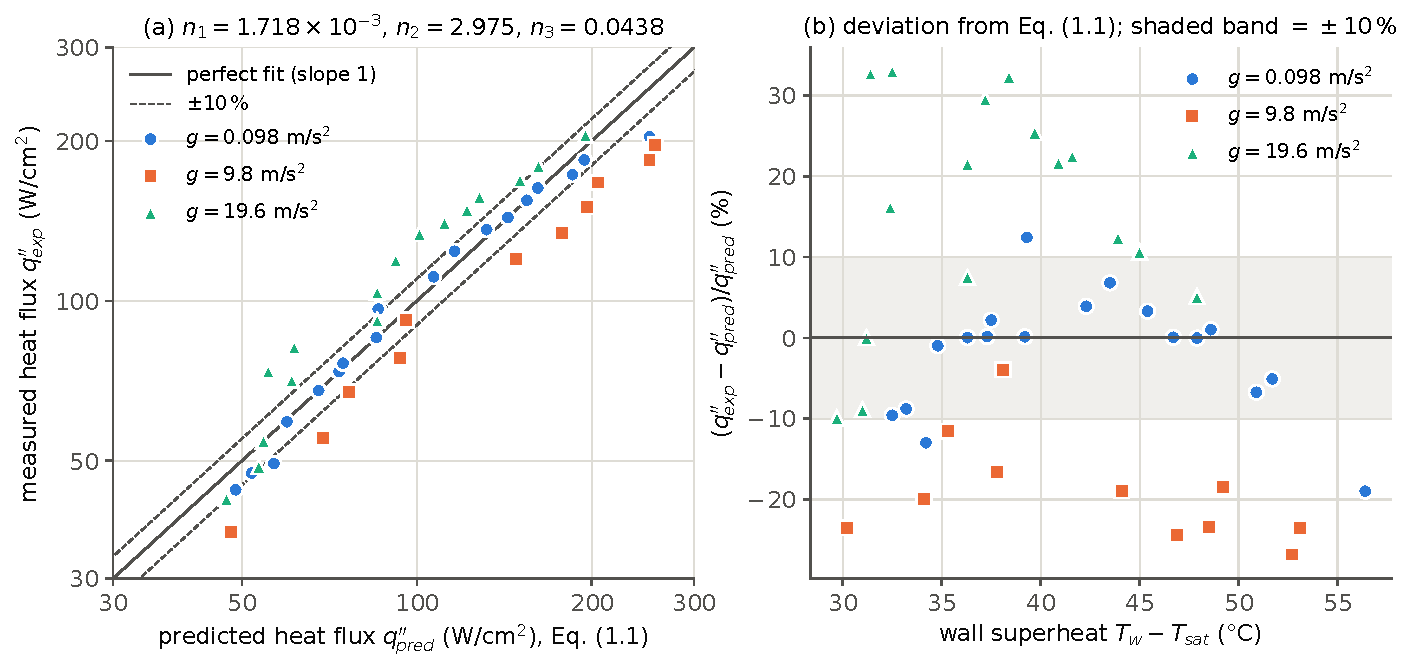
\includegraphics[width=\linewidth]{figures/t22_parity.pdf}
\caption{Task 2.2: (a) measured versus predicted heat flux for the best-fit constants (log-log); (b)
fractional deviation versus superheat. Each gravity level has its own symbol.}
\label{fig:t22parity}
\end{figure}

\paragraph{Assessment of the fit with respect to the $\pm10\,\%$ uncertainty.}
\textbf{The fit is not tighter than the uncertainty of the data}: the rms deviation ($\TwoTwoRmsRel\,\%$) and the
mean absolute deviation ($\TwoTwoMeanAbsRel\,\%$) are larger than the estimated $\pm10\,\%$
measurement uncertainty. The superheat is also uncertain: $\pm0.5$\,\textdegree C at 40\,\textdegree C gives $\pm4\,\%$ on
$\qpp$ through $n_2\approx3$, so the combined noise is about $10.7\,\%$. That is still clearly below the
rms deviation. \textbf{The deviation of the fit is therefore above the noise level of the data.} The
groups in Fig.~\ref{fig:t22parity}(b) show where it comes from. The deviations are
\emph{systematic}, not random:
\begin{center}\small
\begin{tabular}{@{}l c c@{}}
\toprule
Group & mean deviation & rms deviation\\
\midrule
$g=0.098$~m/s$^2$ (18 points) & $\TwoTwoBiasLow\,\%$  & $\TwoTwoRmsLow\,\%$\\
$g=9.8$~m/s$^2$ (11 points)   & $\TwoTwoBiasMid\,\%$  & $\TwoTwoRmsMid\,\%$\\
$g=19.6$~m/s$^2$ (16 points)  & $\TwoTwoBiasHigh\,\%$ & $\TwoTwoRmsHigh\,\%$\\
\bottomrule
\end{tabular}
\end{center}
The $0.01\,\gen$ group is fitted to within the noise ($7.5\,\%$ rms). The $1\,\gen$ group is overpredicted
by about $19\,\%$ and the $2\,\gen$ group underpredicted by about $16\,\%$. With a single exponent, $g^{n_3}$
cannot represent at the same time an almost zero change between $0.01$ and $1\,\gen$ (Task~2.1(b)) and a
$15$--$30\,\%$ increase between $1$ and $2\,\gen$, so $n_3$ ends up as a compromise. This is a
\textbf{model-form error}: the Marangoni contribution, which keeps the heat flux finite when $g\to0$, is
missing from Eq.~(1.1).

Consequences for the use of Eq.~(1.1):
\begin{itemize}
  \item \emph{Accuracy of the predictions}: a heat flux predicted by Eq.~(1.1) is uncertain by about
        $\pm17\,\%$ (one standard deviation), and up to $\pm30\,\%$ for some conditions. This is larger
        than the measurement uncertainty and depends on the gravity level (biased predictions at
        $1\,\gen$ and $2\,\gen$).
  \item \emph{Accuracy of the predicted trends}: the superheat trend ($n_2\approx3$) is robust. It agrees
        with Task~2.1(b) and changes little between the runs. The gravity trend is not reliable: the
        model predicts that $\qpp$ increases by $100^{n_3}-1\approx22\,\%$ between $0.01\,\gen$ and
        $1\,\gen$, while the data show almost no change. Extrapolating to $g\to0$ would even predict
        $\qpp\to0$, which is the opposite of the observed Marangoni behaviour.
  \item To bring the deviation down to the noise level, the model must contain the missing physics. The
        five-constant model of Task~2.3 adds it, and removes most (not all) of this bias.
\end{itemize}
